\documentclass[12pt,a4paper]{article}

\usepackage[utf8]{inputenc}
\usepackage[T1]{fontenc}
\usepackage[top=2.5cm,bottom=2.5cm,left=2.5cm,right=2.5cm]{geometry}
\usepackage{booktabs}
\usepackage{longtable}
\usepackage{array}
\usepackage{graphicx}
\usepackage[colorlinks=true,linkcolor=blue,citecolor=blue,urlcolor=blue]{hyperref}
\usepackage{url}
\usepackage{textcomp}
\usepackage{caption}
\usepackage{subcaption}
\usepackage{authblk}
\usepackage[numbers,sort&compress]{natbib}
\usepackage{setspace}
\usepackage{titlesec}
\usepackage{float}
\usepackage{multirow}

\titleformat{\section}{\large\bfseries}{}{0em}{}
\titleformat{\subsection}{\normalsize\bfseries}{}{0em}{}
\titleformat{\subsubsection}{\normalsize\itshape}{}{0em}{}

\setlength{\parskip}{6pt}
\setlength{\parindent}{0pt}

\graphicspath{{figures/}}

\newcommand{\feat}[1]{\texttt{#1}}

% ============================================================
\title{\textbf{ERGON: A Grambank-Inspired Database for the\\
Quantitative Typological Study of Ergativity}}

\author[1,3,*]{Roberto Zariquiey}
\author[1]{Jaime Montoya}
\author[1]{Luisa G\'{o}mez}
\author[1]{Claudia Alvarado}
\author[1]{Santiago Chu Pr\'{i}ncipe}
\author[2,1]{Leslie Lanasca}
\author[5]{Ana\'{i}s Almendra}
\author[1,4]{Mariana Poblete}
\author[6,3]{Simon Greenhill}
\author[3]{Russell D. Gray}

\affil[1]{Estaci\'{o}n Cient\'{i}fica Chana para las Ciencias del Lenguaje y la
  Interculturalidad, Departamento de Humanidades, Pontificia Universidad
  Cat\'{o}lica del Per\'{u} (PUCP), Lima, Per\'{u}}
\affil[2]{Universidad Nacional Mayor de San Marcos, Lima, Per\'{u}}
\affil[3]{Department of Linguistic and Cultural Evolution, Max Planck
  Institute for Evolutionary Anthropology, Leipzig, Germany}
\affil[4]{Leiden University, Leiden, The Netherlands}
\affil[5]{Universidad de Chile, Santiago, Chile}
\affil[6]{University of Auckland}
\affil[*]{Correspondence:
  \href{mailto:rzariquiey@pucp.edu.pe}{rzariquiey@pucp.edu.pe}}

\date{}

% ============================================================
\begin{document}
\maketitle

\noindent\textbf{Abstract}

ERGON is a cross-linguistic typological database documenting patterns of ergative alignment of flagging across 177 ergative languages from 40 language families. Directly inspired by Grambank \cite{grambank2023} and its feature GB409 (\textit{Is there any ergative alignment of flagging?}), ERGON expands this single binary variable into 24 sub-features (GB409\_1--GB409\_24) that capture the full structural complexity of ergative flagging: its distribution across the person and animacy hierarchy, its conditioning by aspect, tense, mood, realis status, agentivity, topicality, and clause type, and its formal overlap with other case categories. The database contains 4,104 coded binary values distributed across 196 languages (177 ergative, 13 non-ergative controls, 6 problematic) and is formatted as a Cross-Linguistic Data Format (CLDF) StructureDataset \cite{forkel2018}, ensuring interoperability with Glottolog, WALS, Grambank, and other typological resources. A structured curation protocol involving expert review against primary grammar sources yielded corrections across multiple languages; the full curation methodology is described in a companion paper \cite{zariquiey2026curation}. ERGON is publicly available at \url{https://github.com/rzariquiey/ergon-database}.

\medskip
\noindent\textbf{Keywords:} ergativity, typology, cross-linguistic database,
CLDF, Grambank, ergative flagging, split ergativity, Silverstein hierarchy

% ============================================================
\section{Background \& Summary}

Ergativity is one of the most theoretically significant and cross-linguistically diverse phenomena in linguistic typology. In an ergative alignment pattern, the sole argument of an intransitive clause (S) is treated morphosyntactically in the same way as the patient of a transitive clause (P), rather than the transitive agent (A). This contrasts with the more widespread nominative-accusative pattern, in which S is grouped with A to the exclusion of P \cite{dixon1994,comrie1978}. Languages of the world display an enormous range of alignment strategies, with nominative-accusative, ergative-absolutive, tripartite, and active-stative systems representing only the most commonly discussed types \cite{witzlackmakarevich2019}. Ergative alignment is particularly intriguing because of its cross-linguistic variability: while the nominative-accusative pattern tends to be applied uniformly across a language's grammar, ergative alignment is frequently restricted to specific grammatical domains --- certain person categories, tense-aspect values, clause types, or nominal categories --- giving rise to the phenomenon known as ``split ergativity'' \cite{dixon1994,silverstein1976}.

Ergative alignment may be realised through at least three distinct morphosyntactic mechanisms: case marking on nominal arguments (flagging), cross-referencing affixes on the verb (indexing), and syntactic pivot constraints that determine which argument can be omitted, relativised, or coordinated across clauses \cite{dixon1994,manning1996}. These three domains of ergativity are logically independent: a language may display ergative flagging without ergative indexing, or vice versa \cite{siewierska2005}. The present database is concerned exclusively with ergative alignment of \textit{flagging} --- that is, differential case marking on NPs and pronouns that groups S with P (absolutive) in opposition to A (ergative). This focus on flagging follows the operationalisation adopted by Grambank \cite{grambank2023} in its feature GB409 and reflects the theoretical primacy of case marking in the typological literature on ergativity, where the presence or absence of ergative case markers on different nominal categories constitutes the primary evidence for the Silverstein hierarchy \cite{silverstein1976} and for split-ergativity typologies \cite{dixon1994,givon2001}.

The distinction between flagging and indexing is crucial for the proper coding of ergativity and has been the source of considerable analytical confusion in the typological literature. Flagging refers to case markers that attach to NPs and free pronouns, whereas indexing refers to bound pronominal affixes that cross-reference arguments on the verb \cite{haspelmath2013,nichols1986}. Nichols's \cite{nichols1986} foundational distinction between ``head-marking'' and ``dependent-marking'' grammar provides the conceptual basis for this separation: flagging is dependent-marking (the case marker appears on the dependent NP), while indexing is head-marking (the pronominal affix appears on the verbal head). Many languages described as ``ergative'' in the literature exhibit ergative alignment only in their verbal indexing system, with free NPs and pronouns showing no case distinction or following a nominative-accusative pattern. This is particularly common in western Austronesian languages, where pronominal clitics attached to the verb may display an ergative-absolutive distribution while free nominals carry no case marking at all \cite{liao2004,aldridge2004}. ERGON codes only flagging-based ergativity, following the operationalisation of Grambank's GB409, which explicitly targets ``ergative alignment of flagging.'' Languages whose sole ergative alignment is realised through verbal indexing are coded as 0 (absent) on the relevant ERGON features.

Existing large-scale typological databases provide only a starting point for studying the internal diversity of ergative systems. The World Atlas of Language Structures (WALS) \cite{dryer2013} includes features relevant to case alignment --- notably feature 98A (``Alignment of Case Marking of Full Noun Phrases'') and feature 99A (``Alignment of Case Marking of Pronouns'') --- but these features classify languages into broad alignment types (ergative, accusative, tripartite, etc.) without further differentiation within the ergative category. A language with ergative marking restricted to full NPs in the perfective aspect and a language with pervasive ergative marking across all persons, tenses, and clause types both receive the same ``ergative'' classification. Moreover, WALS features 98A and 99A are coded for a relatively small sample of languages and do not capture the conditioning factors --- tense, aspect, mood, agentivity, topicality --- that are central to the theoretical analysis of split ergativity.

Grambank \cite{grambank2023}, the most comprehensive binary-feature typological database to date --- covering 195 features for over 2,400 languages --- represents a substantial advance in cross-linguistic coverage. Grambank's feature GB409 (``Is there any ergative alignment of flagging?'') identifies the presence of ergative case marking at the language level and has enabled important large-scale comparative analyses, including investigations of the global distribution of ergativity and its genealogical and areal correlates \cite{skirgard2023}. However, the binary nature of GB409 necessarily collapses the rich internal variation found within ergative systems. A language that marks the ergative only on third-person full NPs in the perfective aspect of main clauses receives the same code (1 = present) as a language with pervasive ergative marking across all persons, tenses, aspects, moods, and clause types. This loss of information is unavoidable in a database designed for maximal breadth, but it means that fine-grained typological questions about the \textit{structure} of ergativity --- where it occurs, under what conditions, and with what formal properties --- cannot be addressed using Grambank alone.

ERGON was designed precisely to fill this gap. Taking Grambank's GB409 as its point of departure, ERGON expands this single feature into 24 binary sub-features (GB409\_1--GB409\_24) that together document whether ergative alignment of flagging is present across a range of structural domains. The 24 features cover the distribution of ergative marking across the person/animacy hierarchy (1st, 2nd, 3rd person pronouns, full NPs), its conditioning by aspect (perfective vs.\ imperfective), tense (past vs.\ non-past), mood (indicative vs.\ non-indicative), realis status (realis vs.\ irrealis), semantic properties of the agent (agentivity, topicality, animacy), clause type (main vs.\ non-main), and formal properties of the ergative marker (overlap with genitive, instrumental, or comitative). Like Grambank, ERGON adopts a strictly binary coding scheme and distributes its data in CLDF format \cite{forkel2018}, ensuring compatibility with Grambank, Glottolog \cite{hammarstrom2024}, Lexibank \cite{list2022}, and the broader ecosystem of CLDF-compatible typological resources. ERGON can thus be understood as a domain-specific extension of the Grambank model: where Grambank provides the broadest possible cross-linguistic coverage, ERGON provides depth of coverage within a single, theoretically rich phenomenon.

The current release covers 177 ergative languages from 40 language families, with an additional 13 non-ergative languages included as typological controls and 6 languages flagged as problematic (Figure~\ref{fig:map}). The geographic distribution of the sample spans all inhabited continents and major linguistic areas, with particularly dense coverage in the Himalayan region and mainland Southeast Asia (Trans-Himalayan family, 43 languages), the Philippines and Oceania (Austronesian, 33 languages), Australia (Pama-Nyungan, 24 languages), the highlands of New Guinea (Trans-New Guinea, 18 languages), and lowland South America (Panoan, 7 languages; Cariban, 2 languages). The database also includes representatives of the Caucasian families (Nakh-Daghestanian, Kartvelian), the Eskimo-Aleut family, several language isolates (Basque, Burushaski), and diverse smaller families across North America, Africa, and the Pacific. This broad geographic and genealogical coverage ensures that the patterns documented in ERGON are not artefacts of sampling bias toward particular regions or lineages.

The database contains 4,104 coded binary values across 24 features, with 579 values coded as missing (?). All data underwent a structured expert curation protocol against primary grammar sources. The curation process revealed and corrected several types of coding errors, including languages whose ``ergative'' marking was realised through verbal indexing rather than case flagging, languages where the marker described as ergative was in fact an optional agentivity marker, and languages where the hierarchy patterns were inconsistent with the source grammar evidence. The database supports quantitative research on the Silverstein animacy/person hierarchy \cite{silverstein1976}, split ergativity conditioned by tense, aspect, mood, and realis \cite{dixon1994,givon2001}, feature co-occurrence patterns \cite{bybee1994}, formal overlap between the ergative and other case categories \cite{blake2001}, and phylogenetic signal in ergativity distributions \cite{greenhill2010,blasi2019}.

% ============================================================
\section{Methods}

\subsection{Language sample}

The language sample was assembled primarily on the basis of Grambank \cite{grambank2023}. Grambank feature GB409 --- ``Is there any ergative alignment of flagging?'' --- identifies languages with ergative case marking across the full Grambank sample of over 2,400 languages. From this universe, 196 languages were selected for ERGON, with the aim of covering all major linguistic macro-areas and a significant portion of the world's genealogical families that exhibit ergative alignment of flagging, with particular emphasis on families for which existing typological databases have had limited coverage.

The selection was guided by three criteria. First, genealogical breadth: the sample aims to include representatives of as many language families with attested ergative flagging as possible, in order to minimise the risk of conflating genealogical inheritance with typological tendency. Second, geographic coverage: languages were selected to cover all major macro-areas (Africa, Eurasia, Papunesia, Australia, North America, South America) in order to permit areal analyses. Third, availability of descriptive sources: only languages for which a published reference grammar or substantial grammatical sketch was available were included, as the coding of 24 binary features requires detailed information about case marking across a range of grammatical contexts. The selection was supplemented by expert judgement to ensure representation of language groups documented primarily through primary fieldwork and descriptive literature, including several Panoan and Takanan languages of Amazonian South America that are absent from or insufficiently represented in existing large-scale databases.

During the annotation process, 13 of the initially selected languages were found not to display clear ergative alignment of flagging upon consultation of primary sources. In some cases, the language had been classified as ergative in Grambank on the basis of verbal indexing patterns rather than case marking on NPs; in other cases, the source grammar was ambiguous or the alignment pattern was better classified as active-stative rather than ergative. Rather than excluding them, these languages were retained in ERGON as a non-ergative control group, coded as 0 on all 24 features. This control group serves two purposes: it provides a baseline for validation analyses, and it documents cases where the boundary between ergative and non-ergative classification is genuinely unclear. An additional 6 languages were flagged as ``problematic'' due to unresolvable classification issues, such as conflicting descriptions in different source grammars or features of the alignment system that do not fit neatly into the ergative/non-ergative binary.

Each language is identified by its Glottocode \cite{hammarstrom2024} as a stable, database-independent identifier that links ERGON entries unambiguously to the Glottolog catalogue and, through it, to other CLDF-compatible databases. The final ERGON sample comprises 177 ergative languages from 40 families, 13 non-ergative control languages, and 6 problematic languages (Table~\ref{tab:families}; Figure~\ref{fig:map}).

\subsection{Feature design}

The 24 ERGON features are all sub-features of Grambank's GB409, operationalised as binary questions about the presence (1) or absence (0) of ergative alignment of flagging in a specific structural domain. Table~\ref{tab:features} presents all 24 features with their definitions and coverage rates in the ergative subsample. The design of the feature set was informed by the major theoretical frameworks for analysing split ergativity and by the range of conditioning factors documented in the descriptive literature on ergative languages.

The feature set is organised into seven thematic groups:

\begin{enumerate}
\item \textbf{Baseline} (GB409\_1): presence of an overt absolutive marker. While most ergative languages treat the absolutive as the unmarked case (zero-marked), a minority employ an overt absolutive suffix or clitic. This feature captures this typologically significant distinction, which has implications for the formal analysis of ergativity and for the diachronic origins of ergative case systems \cite{mcgregor2009}.

\item \textbf{Person/animacy hierarchy} (GB409\_2--5): ergative flagging on first person pronouns, second person pronouns, third person pronouns, and full NPs, respectively. These four features jointly operationalise the Silverstein hierarchy \cite{silverstein1976}, one of the most robust implicational universals in morphological typology. The hierarchy predicts that ergative marking is more likely on full NPs than on pronouns, and more likely on third person than on first or second person, reflecting the functional principle that arguments higher on the animacy/definiteness scale are more likely to be agents and therefore less in need of explicit agent marking \cite{comrie1989,aissen2003}.

\item \textbf{Aspect} (GB409\_6--7): ergative flagging in the imperfective and perfective aspects. Aspect-conditioned splits, in which ergative marking is restricted to the perfective or completive aspect, are among the best-documented types of split ergativity \cite{dixon1994}. The classic analysis, going back to \cite{dixon1979}, links this split to the semantic affinity between the perfective viewpoint and the transitivity of the event: completed events foreground the distinction between agent and patient, making ergative marking functionally more relevant.

\item \textbf{Tense} (GB409\_8--9): ergative flagging in the past tense and in non-past tenses. Tense-conditioned splits are closely related to aspect-conditioned splits, since past tense and perfective aspect frequently co-occur or are formally fused in the world's languages \cite{bybee1994}. In many languages, including several Indo-Iranian and Tibeto-Burman languages, ergative marking is restricted to past-tense or perfective clauses, while present and future clauses employ nominative-accusative alignment \cite{verbeke2013}.

\item \textbf{Mood/realis} (GB409\_10--13): ergative flagging in the indicative mood, non-indicative moods, realis status, and irrealis status. These features capture a broader set of conditioning contexts related to the epistemic and modal properties of the clause. Mood-conditioned splits, while less commonly discussed than aspect splits, have been documented in a number of language families, including Tibeto-Burman \cite{delancey1981} and Eskimo-Aleut \cite{miyaoka2012}.

\item \textbf{Agentivity, topicality, animacy of A} (GB409\_14--19): ergative flagging conditioned by the semantic properties of the transitive agent argument: agentive vs.\ non-agentive, topical vs.\ non-topical, animate vs.\ inanimate. These features address the role of discourse-pragmatic and semantic factors in conditioning ergativity, following proposals by \cite{givon2001} and \cite{duBois1987} that ergative marking is sensitive to the information-structural status of the agent. In some languages, the ergative marker is omitted when the agent is topical, given, or highly agentive, suggesting that ergativity functions as a device for marking non-canonical or unexpected agents rather than agents per se \cite{mcgregor2010}.

\item \textbf{Clause type, other factors, and formal overlap} (GB409\_20--24): ergative flagging in main clauses, non-main clauses, other conditioning contexts, and formal identity of the ergative marker with the genitive (GB409\_23) or instrumental/comitative (GB409\_24). The clause-type features capture the well-documented tendency for ergative marking to be restricted to main clauses in some languages, with subordinate and relative clauses displaying nominative-accusative or neutral alignment \cite{dixon1994}. The formal-overlap features address the diachronic origins of ergative markers: the syncretic identity of the ergative with the instrumental case is one of the best-known pathways of ergative development, arising from passive or antipassive reanalyses \cite{garrett1990,estival1985}, while ergative-genitive syncretism is characteristic of languages where the ergative case developed from a possessive construction \cite{blake2001}.
\end{enumerate}

All features were coded as binary: 1 if the described pattern is present in the language, 0 if it is absent, and ? if the available sources did not provide sufficient information for a coding decision. Crucially, only \textit{flagging} --- case marking on NPs and free pronouns --- is coded. Ergative alignment realised exclusively through verbal indexing (bound pronominal affixes on the verb) does not count as ergative flagging and is coded as 0. This distinction is particularly important for several Austronesian languages (e.g., Bugis, Pitu Ulunna Salu) whose ergative alignment is realised through pronominal proclitics and enclitics on the verb rather than through case markers on nominal arguments \cite{liao2004}.

\subsection{Data collection}

Feature values were coded by the principal investigator and a team of research assistants, drawing exclusively on published descriptive grammars and, where available, on fieldwork notes and primary data collected by the principal investigator. For each language, the coder consulted the most comprehensive available reference grammar, prioritising recent and detailed descriptions over older or more schematic sources. In cases where multiple grammars or grammatical sketches were available for the same language, all available sources were consulted, with priority given to the most recent and comprehensive description. Values were entered into individual language coding sheets (\textit{fichas}) in spreadsheet format, one row per feature, with columns for the feature identifier, the coded value, the bibliographic source, page reference, and a free-text comment field for disambiguation.

The coding process required careful attention to the distinction between flagging and indexing, between obligatory case markers and optional or discourse-conditioned markers, and between true ergative-absolutive alignment and superficially similar patterns such as differential agent marking or optional agent flagging. Coders were instructed to code a feature as 1 only if the source grammar provided clear evidence of a dedicated case marker or clitic that attaches to NPs or free pronouns and that distinguishes A from S arguments. Where the source grammar was ambiguous or where the described pattern could be analysed as either ergative flagging or indexing, the coder flagged the value as uncertain in the comment field and the case was reviewed by the principal investigator.

The raw dataset comprised 157 Excel fichas, 38 CSV fichas, and 222 PDF reference grammars, covering 196 languages across two source archives. Languages are distributed across two categories in the repository: \textbf{original} files containing the initial codings as entered by the coder, and \textbf{curated} files containing the post-review values. Where a curated file exists for a language, it takes priority over the original file in the CLDF build pipeline.

\subsection{Curation protocol}

The ERGON data underwent a systematic, multi-stage curation process documented in full in \cite{zariquiey2026curation}. The curation protocol was designed to identify and correct errors at multiple levels --- from file-level metadata issues to feature-level coding decisions --- and to ensure that every coded value is supported by explicit textual evidence from the source grammar. The protocol involved the following steps:

\begin{enumerate}
\item \textbf{File extraction and normalisation}: all source fichas (both Excel and CSV formats) were extracted, parsed with automatic delimiter detection, and converted to a standardised tabular format with consistent column names.

\item \textbf{Metadata enrichment}: systematic addition of language-level metadata (Glottocode, language name, genealogical family) to all tabular records, linking each ficha to Glottolog for cross-database interoperability.

\item \textbf{Filename standardisation}: all filenames were standardised to Glottocodes to ensure a one-to-one mapping between files and languages.

\item \textbf{Error detection and classification}: a battery of automated and manual checks identified three types of data quality issues: Type 1 errors (Glottocode filename corresponding to a different language than the one documented in the ficha), Type 2 errors (initially unresolved language identity, subsequently resolved through consultation of Glottolog and source grammars), and Type 3 errors (unresolvable discrepancies between the Glottocode, the language name, and the grammatical source).

\item \textbf{Feature-level verification}: coded values were systematically verified against primary source PDFs, with particular attention to the Silverstein hierarchy features (GB409\_2--5), which have the highest theoretical significance and the greatest risk of coding error due to the common conflation of flagging and indexing in descriptive grammars.

\item \textbf{Expert review of Silverstein patterns}: all languages coded as (1,1,1,1) on the hierarchy features --- indicating ergative marking across all person categories and full NPs --- were individually reviewed against source grammars by the principal investigator. This review identified several categories of coding errors: languages where the ``ergative'' marking was not a proper case marker but an optional agentivity marker (e.g., Kamula, where the putative ergative suffix is an optional agent-emphasis marker that can also appear on intransitive subjects); languages where the marker described as ergative was not obligatory or did not clearly distinguish A from S (e.g., Futuna-Aniwa); and languages where the ergative alignment was realised through verbal indexing rather than case flagging (e.g., Bugis, where Hanson \cite{hanson2003} describes ``ergative proclitics'' that are in fact bound pronominal prefixes cross-referencing agents on the verb, and Pitu Ulunna Salu, where Campbell \cite{campbell1989} explicitly states that ``there are no case markings on nouns'' and that ``absolutive/ergative case inflections are limited to the arguments represented by pronominal affixes on the verb stem'').
\end{enumerate}

All corrections are documented in the \texttt{values.csv} file through the Comment field, which preserves the textual evidence from the source grammar supporting each coding decision. This ensures full transparency and reproducibility: any user can verify any coding decision by consulting the cited page of the referenced grammar.

\subsection{CLDF build pipeline}

The CLDF dataset was assembled from the curated language files using a dedicated build script (\texttt{build\_cldf.py}), available in the repository root. The pipeline performs the following operations: (1) it scans the curated and original data directories, giving priority to curated files where both exist for the same language; (2) it parses each file with automatic delimiter detection, handling both comma-separated and tab-separated formats; (3) it extracts the 24 coded feature values and associated metadata (source, comment) for each language; (4) it validates each language identifier against the Glottocode regular expression \texttt{[a-z]\{4\}[0-9]\{4\}}; and (5) it writes CLDF-compliant \texttt{languages.csv}, \texttt{parameters.csv}, and \texttt{values.csv} tables, together with a \texttt{StructureDataset-metadata.json} file declaring the CLDF conformance profile, column definitions, and foreign key constraints. The entire pipeline is deterministic and can be re-run from the raw source files to regenerate the CLDF dataset.

% ============================================================
\section{Data Records}

The ERGON dataset is distributed as a CLDF StructureDataset \cite{forkel2018} hosted at \url{https://github.com/rzariquiey/ergon-database}. The CLDF format was chosen because it provides a standardised, machine-readable structure for cross-linguistic typological data that is interoperable with the major typological databases (Grambank, WALS, Lexibank, CLICS) and with the Glottolog language catalogue \cite{hammarstrom2024}. The CLDF dataset is located in the \texttt{cldf/} directory and consists of the following files.

\textit{languages.csv.} One row per language ($n = 196$). Columns: \texttt{ID} (Glottocode), \texttt{Name} (language name as given in Glottolog), \texttt{Glottocode} (same as ID, included for CLDF compatibility), \texttt{Family} (top-level genealogical unit following the classification in Glottolog 5.0), and \texttt{Ergative\_type} (\texttt{ergative}, \texttt{non\_ergative}, or \texttt{problematic}). The file contains 196 rows: 177 ergative languages from 40 families, 13 non-ergative control languages, and 6 problematic languages (Table~\ref{tab:families}).

\textit{parameters.csv.} One row per feature ($n = 24$). Columns: \texttt{ID} (e.g.\ \feat{GB409\_1}), \texttt{Name} (same as ID), \texttt{Description} (full feature question as listed in Table~\ref{tab:features}). The file contains 24 rows corresponding to GB409\_1--GB409\_24. Feature identifiers deliberately follow the Grambank naming convention (GB409 prefix) to make explicit the derivational relationship between ERGON's sub-features and Grambank's parent feature.

\textit{values.csv.} One row per language--feature combination ($n = 4{,}685$). Columns: \texttt{ID} (sequential integer), \texttt{Language\_ID} (Glottocode, foreign key to \texttt{languages.csv}), \texttt{Parameter\_ID} (feature identifier, foreign key to \texttt{parameters.csv}), \texttt{Value} (\texttt{0}, \texttt{1}, or \texttt{?}), \texttt{Source} (bibliographic reference with page numbers), and \texttt{Comment} (free-text annotation documenting the coding rationale and, where applicable, verbatim quotations from the source grammar). Of the 4,685 rows, 4,104 carry a coded binary value (0 or 1) and 579 are coded as missing (?). The Comment field is particularly important for the transparency of the dataset: it records the textual evidence from the source grammar that supports each coding decision, including direct quotations where the coding was non-trivial or where the source grammar's terminology required interpretation (e.g., when a grammar uses the term ``ergative'' to describe what is functionally an indexing rather than a flagging pattern).

\textit{StructureDataset-metadata.json.} A CLDF-compliant metadata file declaring the dataset's conformance to the CLDF StructureDataset profile, column definitions, data types, foreign key constraints, and dataset-level metadata including the dataset DOI, licence, and citation information.

Additional files in the repository include: \texttt{analysis/} (Python analysis scripts, output figures, and derived CSV tables including Silverstein classifications, ergativity scores, and dimensionality scores); \texttt{build\_cldf.py} (the CLDF build script); and \texttt{raw/} (the original and curated source fichas from which the CLDF dataset was built).

% ============================================================
\section{Technical Validation}

\subsection{Feature coverage}

Table~\ref{tab:features} reports feature-level coverage across the 177 ergative languages. Coverage ranges from 68\% (\feat{GB409\_19}, inanimate A; \feat{GB409\_21}, non-main clauses) to 99\% (\feat{GB409\_20}, main clauses). The lowest coverage features correspond to less commonly described conditioning environments (inanimate agents, non-main clauses, topicality, non-agentive A), for which many grammars provide insufficient information. This is a well-known limitation of grammar-based typological databases: not all reference grammars systematically describe case marking in subordinate clauses or with inanimate agents, and the absence of information in a grammar cannot be straightforwardly interpreted as the absence of the phenomenon in the language \cite{skirgard2023}. The highest-coverage features correspond to properties that are straightforward to identify from even brief grammatical descriptions (full NP ergativity, main clause ergativity, ergative marking in the indicative mood).

Figure~\ref{fig:feature_profile} shows the proportion of ergative languages coded as 1 (feature present) for each of the 24 features. Among the features with the highest prevalence rates are: \feat{GB409\_10} (indicative mood, 98\%), \feat{GB409\_20} (main clauses, 97\%), \feat{GB409\_8} (past tense, 97\%), \feat{GB409\_18} (animate A, 97\%), \feat{GB409\_12} (realis, 97\%), \feat{GB409\_7} (perfective, 96\%), \feat{GB409\_14} (agentive A, 96\%), and \feat{GB409\_5} (full NPs, 94\%). These high prevalence rates reflect the fact that most ergative languages maintain their ergative alignment across core grammatical contexts --- indicative main clauses with animate, agentive subjects in the past/perfective --- and that splits typically involve the \textit{loss} of ergativity in marked or peripheral contexts (non-indicative, irrealis, non-main clauses, inanimate or non-agentive agents) rather than its restriction to those contexts.

The lowest prevalence rates are found for \feat{GB409\_23} (ERG=GEN, 33\%), \feat{GB409\_1} (overt absolutive, 37\%), and \feat{GB409\_24} (ERG=INSTR/COM, 51\%). The low rate of overt absolutive marking confirms the well-established typological generalisation that the absolutive case tends to be zero-marked in ergative languages \cite{dixon1994,comrie1978}, with overt absolutive markers being a marked typological option. The variable rates of ergative-genitive and ergative-instrumental syncretism reflect the diverse diachronic origins of ergative case systems: ergative-instrumental syncretism is characteristic of Indo-Iranian, Australian, and some Tibeto-Burman languages where the ergative developed from a passive or antipassive construction \cite{garrett1990}, while ergative-genitive syncretism is found in some Trans-New Guinea and Eskimo-Aleut languages where the ergative may have developed from a possessive/genitive source \cite{blake2001}.

\subsection{Silverstein hierarchy}

A central prediction of the typological literature on ergativity is Silverstein's animacy/person hierarchy \cite{silverstein1976}, which states that ergative marking extends implicationally from lower to higher positions on the hierarchy: full NPs $\to$ 3rd person pronouns $\to$ 2nd person pronouns $\to$ 1st person pronouns. The functional motivation for this hierarchy is that entities higher on the animacy/definiteness scale (1st and 2nd person) are inherently more likely to be agents, and therefore less in need of an explicit morphological marker distinguishing them from patients; conversely, full NPs --- which can refer to any entity regardless of animacy --- benefit more from an overt case distinction between agent and patient roles \cite{comrie1989,aissen2003}. If a language marks the ergative on a higher-animacy category (e.g., 2nd person pronouns), the hierarchy predicts that it should also mark it on all lower-animacy categories (3rd person pronouns and full NPs).

Of 159 ergative languages with complete data on all four hierarchy features (GB409\_2--5), 152 (95.6\%) conform to this implicational constraint. Seven languages exhibit hierarchy violations (Table~\ref{tab:violations}). These violations were individually verified against primary grammar sources during the curation process and constitute genuine typological exceptions rather than coding errors. The violations fall into several types: languages that mark the ergative on pronouns but not on full NPs (e.g., Futuna-Aniwa, Mag-anchi Agta, Narungga), languages that skip an intermediate person category (e.g., Eibela and Jingulu, which mark the ergative on 1st and 2nd person but not 3rd person), and languages with non-contiguous patterns (e.g., Matis, which marks the ergative on 1st person and NPs but not on 2nd or 3rd person pronouns). The existence of these exceptions is consistent with the broader typological literature, which treats the Silverstein hierarchy as a strong statistical tendency rather than an absolute universal \cite{bickel2008}.

The predominant pattern is hier4 (ergative marking on all persons and NPs), found in 100 languages (62.9\% of those with complete data). This finding indicates that the majority of ergative languages in the ERGON sample have a fully generalised ergative case marker that applies uniformly across all nominal categories, without person-based restrictions. The next most frequent patterns are hier3 (NPs only, 23 languages, 14.5\%) and hier2 (3rd person and NPs, 16 languages, 10.1\%), consistent with the Silverstein hierarchy prediction that partial ergative systems preferentially target the lower end of the animacy scale.

Figure~\ref{fig:heatmap} presents a language-by-feature heatmap of the four Silverstein hierarchy features across all ergative languages with complete data, illustrating the predominance of the hier4 pattern and the location of the seven hierarchy violations. Figure~\ref{fig:silverstein_patterns} shows the frequency distribution of all Silverstein pattern categories.

\subsection{Split ergativity patterns}

Split ergativity --- the restriction of ergative marking to specific grammatical contexts --- is a major topic in the typological literature on ergativity \cite{dixon1994,givon2001}. The phenomenon is of both descriptive and theoretical interest: descriptively, it reveals the domains of grammar that interact with case alignment; theoretically, it has been argued to reflect deep functional principles relating to the transitivity of events, the information-structural properties of arguments, and the semantic properties of tense-aspect-mood categories \cite{hopper1980,delancey1981}. ERGON's paired features allow systematic investigation of splits along four conditioning domains: aspect (imperfective vs.\ perfective), tense (past vs.\ non-past), mood (indicative vs.\ non-indicative), and realis status (realis vs.\ irrealis).

Figure~\ref{fig:splits} summarises the distribution of split patterns across these four domains. For the majority of ergative languages, ergative marking is uniform across both members of each pair --- that is, most languages that mark the ergative in the perfective also mark it in the imperfective, and most languages that mark the ergative in the past also mark it in the non-past. This finding nuances the traditional emphasis on tense-aspect splits in the ergativity literature: while such splits are theoretically important and well-attested in certain language families (notably Indo-Iranian and some Tibeto-Burman languages), they are not the predominant pattern cross-linguistically. Most ergative languages maintain their ergative alignment uniformly across the tense-aspect-mood system.

The phi coefficient for \feat{GB409\_8} (past tense) $\times$ \feat{GB409\_7} (perfective) is $\varphi = 0.910$ ($n = 156$), confirming near-perfect co-occurrence and validating the theoretical association between tense and aspect conditioning of ergativity \cite{dixon1994}. This strong correlation is expected on both functional and formal grounds: past tense and perfective aspect frequently co-occur or are formally fused in the world's tense-aspect systems \cite{bybee1994}, and the functional motivations for aspect-conditioned and tense-conditioned splits --- both relating to the foregrounding of event completion and the distinctness of agent and patient roles --- are closely related \cite{hopper1980}.

\subsection{Feature correlations}

Figure~\ref{fig:phi} presents pairwise phi coefficients across all 24 ERGON features. The correlation matrix reveals several important structural patterns in the data. The tense/aspect/mood/realis block (GB409\_6--13) shows very high internal correlations ($\varphi > 0.85$), confirming that ergative marking in one temporal/modal context is a strong predictor of ergative marking in others. This pattern is consistent with the observation that most ergative languages maintain uniform ergative flagging across tense-aspect-mood categories, with splits along these dimensions being the exception rather than the rule. It also suggests that the eight features in this block may be reducible to a smaller number of underlying dimensions, a hypothesis that can be tested through dimensionality reduction techniques such as principal component analysis.

The person features (GB409\_2--4) also correlate highly with each other ($\varphi > 0.70$), forming a coherent cluster that reflects the internal consistency of the Silverstein hierarchy: languages that mark the ergative on one pronominal person category tend to mark it on the others as well. However, the correlations between the person features and \feat{GB409\_5} (full NPs) are notably lower, reflecting the Silverstein hierarchy: many languages mark the ergative on full NPs but not on pronouns, creating an asymmetry that is visible in the correlation structure.

The formal-overlap features (\feat{GB409\_23}, ERG=GEN; \feat{GB409\_24}, ERG=INSTR/COM) show moderate correlations with each other but low correlations with the rest of the feature set, indicating that the formal properties of the ergative marker (its syncretism with other case categories) are largely independent of the distributional properties of ergativity (where and when it appears). This independence is consistent with the view that the formal shape of an ergative marker is determined by its diachronic source, which varies across language families, while its distributional properties reflect synchronic functional pressures that are to some degree universal \cite{blake2001}.

\subsection{Comparison with Grambank}

As a higher-level validation, we compared ERGON's classification of languages as ergative with Grambank's coding of the parent feature GB409 \cite{grambank2023}. For the languages present in both datasets, the vast majority receive consistent classifications: languages coded as ergative in ERGON are coded as 1 (ergative alignment present) in Grambank, and the non-ergative control languages are coded as 0 in Grambank. The few discrepancies reflect three types of situations: (1) the treatment of marginal or split-ergative systems that fall on the boundary of the binary coding and where reasonable coders might disagree; (2) differences in the source grammars consulted, particularly for languages with multiple available descriptions of varying quality; and (3) cases where the ERGON curation process identified the Grambank coding as incorrect (e.g., languages where the ``ergative'' marking described in the consulted grammar is in fact verbal indexing rather than case flagging). These discrepancies are documented in the Comment field of the ERGON \texttt{values.csv} file and contribute to the broader goal of improving the accuracy of cross-linguistic typological databases through iterative expert review.

% ============================================================
\section{Usage Notes}

ERGON is intended for use in quantitative typological research on ergativity and in comparative studies of grammatical diversity. The following considerations should be borne in mind when working with the data.

\textbf{CLDF compatibility.} The dataset can be loaded directly with the \texttt{pycldf} Python library (\url{https://github.com/cldf/pycldf}):

\begin{verbatim}
import pycldf
ds = pycldf.Dataset.from_metadata(
    'cldf/StructureDataset-metadata.json')
\end{verbatim}

\noindent It can also be used with \texttt{cldfbench} \cite{forkel2018} and integrated with Glottolog, WALS, Grambank, and other CLDF resources. The standardised CLDF format means that ERGON data can be joined with Grambank data using shared Glottocodes, enabling analyses that combine ERGON's fine-grained ergativity features with Grambank's broader typological coverage.

\textbf{Flagging vs.\ indexing.} A critical methodological point is that ERGON codes only ergative alignment of \textit{flagging} (case marking on NPs and free pronouns). Languages whose ergative alignment is realised exclusively through verbal indexing (bound pronominal affixes cross-referencing arguments on the verb) are coded as 0 on the relevant features. This is a deliberate design choice, not a limitation: it follows the operationalisation of Grambank's GB409 and reflects the theoretical distinction between flagging and indexing as independent morphosyntactic domains \cite{haspelmath2013,nichols1986}. Users interested in ergative indexing patterns should consult other resources or combine ERGON with indexing-specific datasets. We note that a companion database documenting ergative alignment of indexing is under development and will follow the same CLDF format.

\textbf{Missing values.} 579 values (12.4\% of the total) are coded as~?. These reflect gaps in the available descriptive literature rather than systematic bias: not all reference grammars describe case marking in all the contexts covered by ERGON's 24 features. The distribution of missing values is not random across features (see Table~\ref{tab:features}): features targeting less commonly described contexts (inanimate agents, non-main clauses, topicality) have higher rates of missing data. Analyses should apply appropriate missing-data strategies --- such as pairwise deletion, multiple imputation, or restriction to features with adequate coverage --- and report the number of languages with data for each feature.

\textbf{Genealogical non-independence.} Languages are not independent observations: closely related languages share features through common inheritance rather than independent innovation. The dataset includes family membership information (\texttt{Family} column in \texttt{languages.csv}) to support mixed-effects analyses that control for genealogical signal \cite{jaeger2011} and phylogenetic comparative methods that model trait evolution along language family trees \cite{greenhill2010,blasi2019}. Users should be aware that the ERGON sample is not a balanced genealogical sample: some families (Trans-Himalayan, Austronesian, Pama-Nyungan) are much more densely represented than others, which will influence frequency-based statistics unless appropriate weighting or mixed-effects modelling is applied.

\textbf{Non-ergative and problematic languages.} The 13 non-ergative and 6 problematic languages are included for validation purposes and for analyses that require a contrast group. They should not be treated as representative samples of non-ergative languages, as they were originally selected on the assumption that they would be ergative.

\textbf{Future releases.} ERGON is an ongoing project. Future releases will expand coverage to include additional languages, particularly from under-represented families in Amazonian South America, Papua New Guinea, and sub-Saharan Africa. Source page references for values currently lacking precise citations will also be added incrementally. We welcome contributions from specialists in individual languages or language families; contribution guidelines are available in the repository.

% ============================================================
\section{Code Availability}

All code used to build the CLDF dataset and to conduct the analyses described in the Technical Validation section is available at \url{https://github.com/rzariquiey/ergon-database} under a Creative Commons Attribution 4.0 International Licence (CC BY 4.0). The build script (\texttt{build\_cldf.py}) requires Python $\geq$ 3.9 and the \texttt{pycldf} library. Analysis scripts in \texttt{analysis/} additionally require \texttt{pandas}, \texttt{numpy}, \texttt{matplotlib}, \texttt{seaborn}, and \texttt{scipy}. A master analysis script (\texttt{analysis/run\_all\_v2.py}) regenerates all figures and derived tables from the CLDF source files.

% ============================================================
\section{Data Availability}

The ERGON dataset is openly available at \url{https://github.com/rzariquiey/ergon-database} under a Creative Commons Attribution 4.0 International Licence (CC BY 4.0). A versioned archive will be deposited at Zenodo prior to publication and a permanent DOI assigned. The dataset conforms to the CLDF StructureDataset specification \cite{forkel2018}. All raw source materials (original and curated fichas) are included in the repository for full reproducibility.

% ============================================================
\section*{Acknowledgements}

[To be completed.]

% ============================================================
\section*{Author Contributions}

R.Z. conceived and designed the database, designed the feature set, performed the expert curation, wrote the CLDF build pipeline, conducted the quantitative analyses, and drafted the manuscript. J.M., L.G., C.A., S.C.P., L.L., A.A., and M.P. contributed to data collection, language annotation, and verification of coded values against source grammars. S.G. contributed to the analysis design and provided expertise on phylogenetic comparative methods. R.D.G. supervised the project, provided methodological guidance on quantitative typology, and contributed to the design of the validation analyses. All authors reviewed and approved the final manuscript.

% ============================================================
\section*{Competing Interests}

The authors declare no competing interests.

% ============================================================
% REFERENCES
% ============================================================

\begin{thebibliography}{99}

\bibitem{grambank2023}
Skirg\r{a}rd, H. et al.
Grambank reveals the importance of genealogical constraints on linguistic
diversity and cross-linguistic variation.
\textit{Science Advances} \textbf{9}, eadg6175 (2023).

\bibitem{forkel2018}
Forkel, R. et al.
Cross-Linguistic Data Formats, advancing data sharing and re-use in
comparative linguistics.
\textit{Scientific Data} \textbf{5}, 180205 (2018).

\bibitem{zariquiey2026curation}
Zariquiey, R.
ERGON: A curated cross-linguistic database of ergative alignment features.
Data curation methodology and repository description.
Manuscript (2026). Available at
\url{https://github.com/rzariquiey/ergon-database}.

\bibitem{dixon1994}
Dixon, R. M. W.
\textit{Ergativity}.
Cambridge University Press, Cambridge (1994).

\bibitem{comrie1978}
Comrie, B.
Ergativity. In W. P. Lehmann (ed.), \textit{Syntactic Typology: Studies in
the Phenomenology of Language}, 329--394. University of Texas Press, Austin (1978).

\bibitem{manning1996}
Manning, C. D.
\textit{Ergativity: Argument Structure and Grammatical Relations}.
CSLI Publications, Stanford (1996).

\bibitem{haspelmath2013}
Haspelmath, M.
Argument indexing: A conceptual framework for the syntactic status of bound
person forms. In D. Bakker \& M. Haspelmath (eds.), \textit{Languages Across
Boundaries: Studies in Memory of Anna Siewierska}, 197--226. De Gruyter
Mouton, Berlin (2013).

\bibitem{nichols1986}
Nichols, J.
Head-marking and dependent-marking grammar.
\textit{Language} \textbf{62}, 56--119 (1986).

\bibitem{dryer2013}
Dryer, M. S. \& Haspelmath, M. (eds.)
\textit{The World Atlas of Language Structures Online}.
Max Planck Institute for Evolutionary Anthropology, Leipzig (2013).
\url{https://wals.info}.

\bibitem{hammarstrom2024}
Hammarstr\"{o}m, H., Forkel, R., Haspelmath, M. \& Bank, S.
Glottolog 5.0.
Max Planck Institute for Evolutionary Anthropology, Leipzig (2024).
\url{https://glottolog.org}.

\bibitem{list2022}
List, J.-M. et al.
Lexibank, a publicly available repository of standardized wordlists with
calculated phonological and lexical features.
\textit{Scientific Data} \textbf{9}, 316 (2022).

\bibitem{silverstein1976}
Silverstein, M.
Hierarchy of features and ergativity. In R. M. W. Dixon (ed.),
\textit{Grammatical Categories in Australian Languages}, 112--171.
Australian Institute of Aboriginal Studies, Canberra (1976).

\bibitem{givon2001}
Giv\'{o}n, T.
\textit{Syntax: An Introduction}, Vol.~1.
John Benjamins, Amsterdam (2001).

\bibitem{bybee1994}
Bybee, J., Perkins, R. \& Pagliuca, W.
\textit{The Evolution of Grammar: Tense, Aspect, and Modality in the
Languages of the World}.
University of Chicago Press, Chicago (1994).

\bibitem{greenhill2010}
Greenhill, S. J., Atkinson, Q. D., Meade, A. \& Gray, R. D.
The shape and tempo of language evolution.
\textit{Proceedings of the Royal Society B} \textbf{277}, 2443--2450 (2010).

\bibitem{blasi2019}
Blasi, D. E., Michaelis, S. M. \& Haspelmath, M.
Grammars are robustly transmitted even during the disruption of the
transmission chain.
\textit{Nature Human Behaviour} \textbf{3}, 1268--1278 (2019).

\bibitem{dixon1979}
Dixon, R. M. W.
Ergativity.
\textit{Language} \textbf{55}, 59--138 (1979).

\bibitem{siewierska2005}
Siewierska, A.
Alignment of verbal person marking. In M. Haspelmath, M. Dryer, D. Gil \& B. Comrie (eds.),
\textit{The World Atlas of Language Structures}, 406--409. Oxford University Press, Oxford (2005).

\bibitem{witzlackmakarevich2019}
Witzlack-Makarevich, A. \& Bickel, B.
Argument selectors and alignment. In A. Malchukov \& A. Spencer (eds.),
\textit{The Oxford Handbook of Case}, 237--262. Oxford University Press, Oxford (2019).

\bibitem{skirgard2023}
Skirg\r{a}rd, H. et al.
Grambank reveals the importance of genealogical constraints on linguistic
diversity and cross-linguistic variation.
\textit{Science Advances} \textbf{9}, eadg6175 (2023).

\bibitem{liao2004}
Liao, H.-C.
Transitivity and Ergativity in Formosan and Philippine Languages.
PhD dissertation, University of Hawai'i at M\={a}noa (2004).

\bibitem{aldridge2004}
Aldridge, E.
Ergativity and word order in Austronesian languages.
PhD dissertation, Cornell University (2004).

\bibitem{comrie1989}
Comrie, B.
\textit{Language Universals and Linguistic Typology}, 2nd edn.
University of Chicago Press, Chicago (1989).

\bibitem{aissen2003}
Aissen, J.
Differential object marking: Iconicity vs.\ economy.
\textit{Natural Language \& Linguistic Theory} \textbf{21}, 435--483 (2003).

\bibitem{verbeke2013}
Verbeke, S.
\textit{Alignment and Ergativity in New Indo-Aryan Languages}.
De Gruyter Mouton, Berlin (2013).

\bibitem{delancey1981}
DeLancey, S.
An interpretation of split ergativity and related patterns.
\textit{Language} \textbf{57}, 626--657 (1981).

\bibitem{miyaoka2012}
Miyaoka, O.
\textit{A Grammar of Central Alaskan Yupik (CAY)}.
De Gruyter Mouton, Berlin (2012).

\bibitem{duBois1987}
Du Bois, J. W.
The discourse basis of ergativity.
\textit{Language} \textbf{63}, 805--855 (1987).

\bibitem{mcgregor2009}
McGregor, W. B.
Typology of ergativity.
\textit{Language and Linguistics Compass} \textbf{3}, 480--508 (2009).

\bibitem{mcgregor2010}
McGregor, W. B.
Optional ergative case marking systems in a typological-semiotic perspective.
\textit{Lingua} \textbf{120}, 1610--1636 (2010).

\bibitem{hopper1980}
Hopper, P. J. \& Thompson, S. A.
Transitivity in grammar and discourse.
\textit{Language} \textbf{56}, 251--299 (1980).

\bibitem{garrett1990}
Garrett, A.
The origin of NP split ergativity.
\textit{Language} \textbf{66}, 261--296 (1990).

\bibitem{estival1985}
Estival, D. \& Myhill, J.
Formal and functional aspects of the development from passive to ergative systems.
In F. Plank (ed.), \textit{Relational Typology}, 441--491. Mouton de Gruyter, Berlin (1985).

\bibitem{blake2001}
Blake, B.
\textit{Case}, 2nd edn.
Cambridge University Press, Cambridge (2001).

\bibitem{bickel2008}
Bickel, B.
On the scope of the referential hierarchy in the typology of grammatical relations.
In G. Corbett \& M. Noonan (eds.), \textit{Case and Grammatical Relations},
191--210. John Benjamins, Amsterdam (2008).

\bibitem{jaeger2011}
Jaeger, T. F., Graff, P., Croft, W. \& Pontillo, D.
Mixed effect models for genetic and areal dependencies in linguistic typology.
\textit{Linguistic Typology} \textbf{15}, 281--320 (2011).

\bibitem{hanson2003}
Hanson, C.
\textit{A Grammar of Bugis}.
PhD dissertation, La Trobe University (2003).

\bibitem{campbell1989}
Campbell, P. J.
\textit{Some Aspects of Pitu Ulunna Salu Grammar: A Typological Approach}.
MA thesis, University of Texas at Arlington (1989).

\end{thebibliography}

% ============================================================
% TABLES
% ============================================================

\clearpage

\begin{longtable}{llp{6.5cm}rr}
\caption{The 24 ERGON features, their thematic domain, definition, and coverage in the ergative subsample ($n = 177$). $n$ = number of languages with a coded binary value (0 or 1). \% = percentage of the 177 ergative languages with a coded value.}
\label{tab:features}\\
\toprule
\textbf{Feature} & \textbf{Domain} & \textbf{Definition} & $n$ & \% \\
\midrule
\endfirsthead
\multicolumn{5}{l}{\small\textit{(Table \ref{tab:features} continued)}}\\[2pt]
\toprule
\textbf{Feature} & \textbf{Domain} & \textbf{Definition} & $n$ & \% \\
\midrule
\endhead
\bottomrule
\endfoot
\feat{GB409\_1}  & Baseline    & Is there an overt marker for the absolutive?                               & 171 & 97 \\
\feat{GB409\_2}  & Person      & Is there ERG alignment of flagging on 1st person pronouns?                & 167 & 94 \\
\feat{GB409\_3}  & Person      & Is there ERG alignment of flagging on 2nd person pronouns?                & 166 & 94 \\
\feat{GB409\_4}  & Person      & Is there ERG alignment of flagging on 3rd person pronouns?                & 170 & 96 \\
\feat{GB409\_5}  & Person      & Is there ERG alignment of flagging on full NPs?                           & 174 & 98 \\
\feat{GB409\_6}  & Aspect      & Is there ERG alignment of flagging in the imperfective aspect?             & 144 & 81 \\
\feat{GB409\_7}  & Aspect      & Is there ERG alignment of flagging in the perfective aspect?              & 158 & 89 \\
\feat{GB409\_8}  & Tense       & Is there ERG alignment of flagging in the past tense?                     & 166 & 94 \\
\feat{GB409\_9}  & Tense       & Is there ERG alignment of flagging in non-past tenses?                    & 154 & 87 \\
\feat{GB409\_10} & Mood        & Is there ERG alignment of flagging in the indicative mood?                & 166 & 94 \\
\feat{GB409\_11} & Mood        & Is there ERG alignment of flagging in non-indicative moods?               & 135 & 76 \\
\feat{GB409\_12} & Realis      & Is there ERG alignment of flagging in the realis?                         & 163 & 92 \\
\feat{GB409\_13} & Realis      & Is there ERG alignment of flagging in the irrealis?                       & 134 & 76 \\
\feat{GB409\_14} & Agentivity  & Is there ERG alignment of flagging with an agentive A?                    & 165 & 93 \\
\feat{GB409\_15} & Agentivity  & Is there ERG alignment of flagging with a non-agentive A?                 & 127 & 72 \\
\feat{GB409\_16} & Topicality  & Is there ERG alignment of flagging with a topical A?                      & 137 & 77 \\
\feat{GB409\_17} & Topicality  & Is there ERG alignment of flagging with a non-topical A?                  & 123 & 69 \\
\feat{GB409\_18} & Animacy     & Is there ERG alignment of flagging with an animate A?                     & 168 & 95 \\
\feat{GB409\_19} & Animacy     & Is there ERG alignment of flagging with an inanimate A?                   & 120 & 68 \\
\feat{GB409\_20} & Clause type & Is there ERG alignment of flagging in main clauses?                       & 175 & 99 \\
\feat{GB409\_21} & Clause type & Is there ERG alignment of flagging in non-main clauses?                   & 121 & 68 \\
\feat{GB409\_22} & Other       & Is ERG alignment of flagging conditioned by any other factor?             & 137 & 77 \\
\feat{GB409\_23} & Form        & Are the ergative and genitive expressed by the same marker?               & 162 & 92 \\
\feat{GB409\_24} & Form        & Are the ergative and instrumental/comitative expressed by the same marker? & 162 & 92 \\
\end{longtable}

\bigskip

\begin{table}[H]
\centering
\caption{Language families represented in ERGON (ergative languages only, $n = 177$). Families with fewer than 2 languages are grouped as ``Other''.}
\label{tab:families}
\begin{tabular}{lrl}
\toprule
\textbf{Family} & \textbf{Languages} & \textbf{Notes} \\
\midrule
Trans-Himalayan      & 43 & Tibeto-Burman, Qiangic, rGyalrongic subgroups \\
Austronesian         & 33 & Philippine, Oceanic, and other subgroups \\
Pama-Nyungan         & 24 & Australian \\
Trans-New Guinea     & 18 & Large Papuan phylum \\
Panoan               &  7 & Amazonian South America \\
Indo-European        &  6 & Iranian, Armenian, Kurdish, Hindi \\
Nakh-Daghestanian    &  3 & Northeast Caucasus \\
Eskimo-Aleut         &  3 & Arctic; Yupik and Inuit varieties \\
Sino-Tibetan         &  3 & \\
Arandic              &  2 & Australian \\
Cariban              &  2 & Amazonian \\
Daly                 &  2 & Australian (Northern Territory) \\
Language isolate     &  2 & Basque, Burushaski \\
Macro-J\^{e}         &  2 & Brazilian \\
Mirndi               &  2 & Australian \\
Other (25 families)  & 25 & One language per family \\
\midrule
\textbf{Total}       & \textbf{177} & \\
\bottomrule
\end{tabular}
\end{table}

\bigskip

\begin{table}[H]
\centering
\caption{Silverstein hierarchy violations in ERGON ($n = 7$ out of 159 languages with complete data on GB409\_2--5). Pattern format: (1st, 2nd, 3rd, NP). All violations were verified against primary grammar sources.}
\label{tab:violations}
\begin{tabular}{llll}
\toprule
\textbf{Language} & \textbf{Glottocode} & \textbf{Family} & \textbf{Pattern} \\
\midrule
Eibela         & aime1238 & Bosavi          & (1, 1, 0, 1) \\
Akuntsu        & akun1241 & Tupian          & (1, 1, 0, 0) \\
Jingulu        & djin1251 & Mirndi          & (1, 1, 0, 1) \\
Futuna-Aniwa   & futu1245 & Austronesian    & (1, 1, 1, 0) \\
Mag-anchi Agta & maga1263 & Austronesian    & (1, 1, 1, 0) \\
Matis          & mati1255 & Panoan          & (1, 0, 0, 1) \\
Narungga       & naru1238 & Pama-Nyungan    & (1, 1, 1, 0) \\
\bottomrule
\end{tabular}
\end{table}

% ============================================================
% FIGURES
% ============================================================

\clearpage

\begin{figure}[H]
\centering
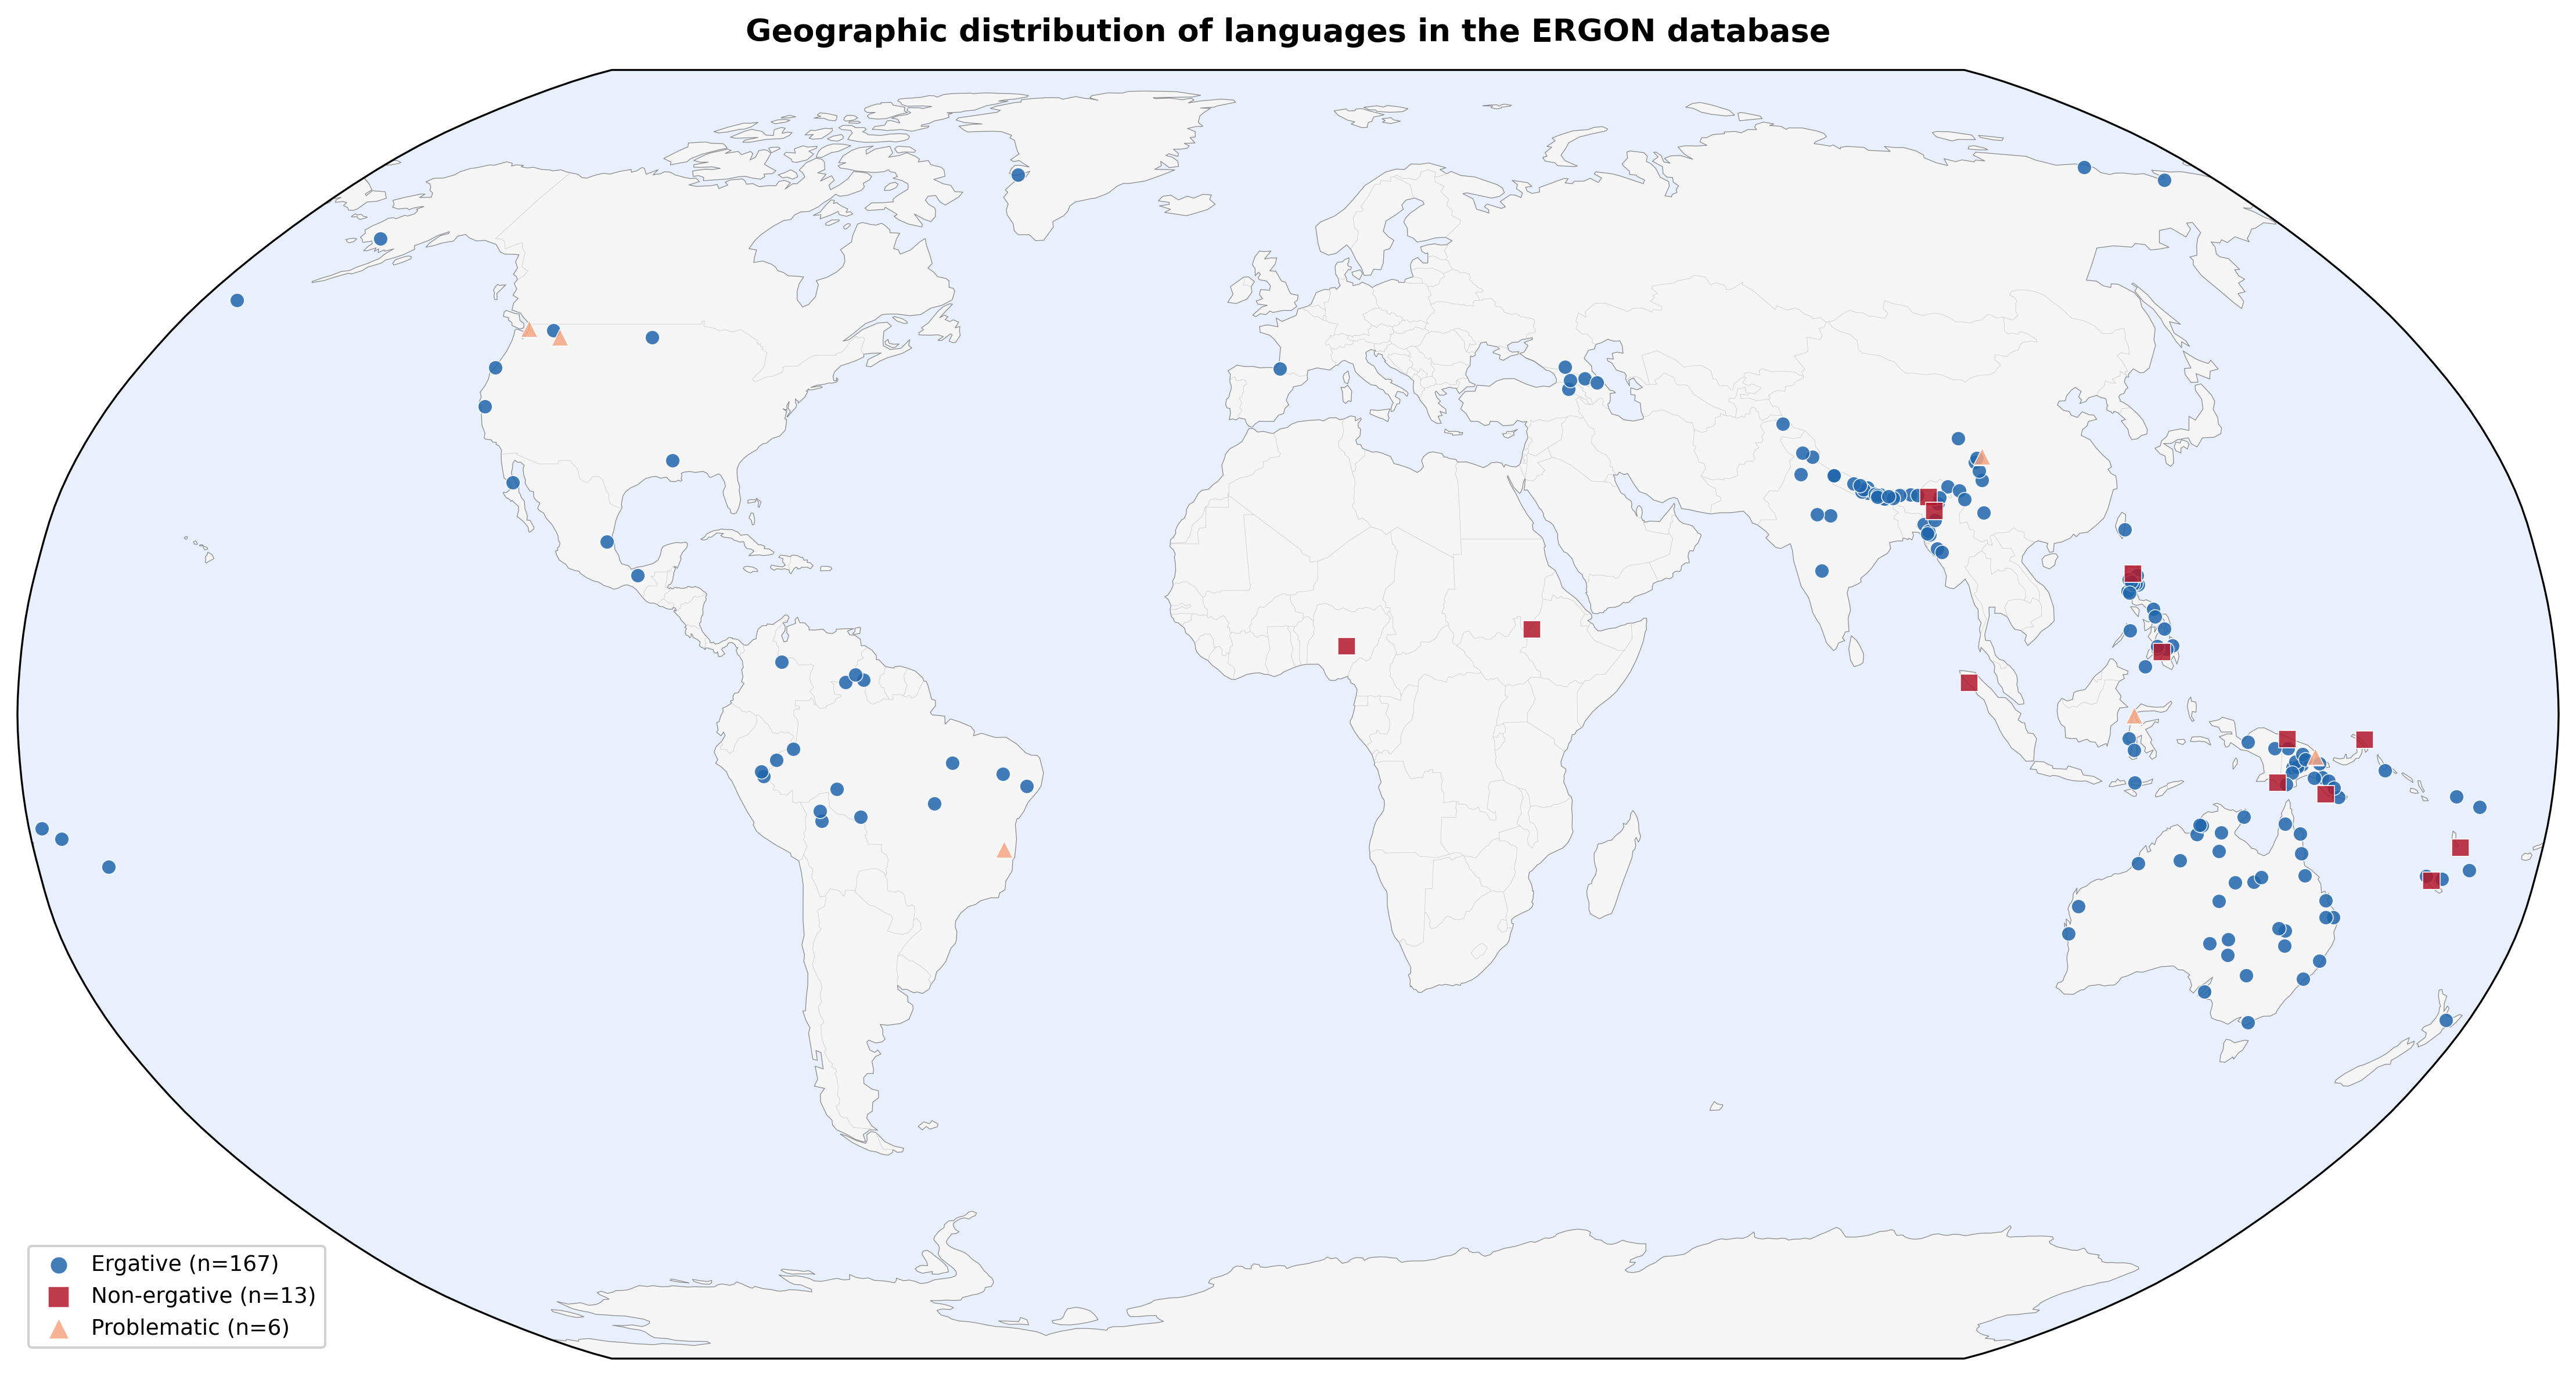
\includegraphics[width=\textwidth]{fig0_language_map.png}
\caption{\textbf{Geographic distribution of languages in the ERGON database.}
Robinson projection map showing the locations of all 186 ERGON languages with
available geographic coordinates (out of 196 total). Blue circles: ergative
languages ($n = 167$); red squares: non-ergative control languages ($n = 13$);
orange triangles: problematic languages ($n = 6$). Coordinates were obtained
from Glottolog 5.0 \cite{hammarstrom2024}. The sample covers all inhabited
continents, with particularly dense coverage in the Himalayan region,
the Philippines, Australia, Papua New Guinea, and Amazonian South America.}
\label{fig:map}
\end{figure}

\begin{figure}[H]
\centering

\includegraphics[width=0.92\textwidth]{fig4_feature_profile.png}
\caption{\textbf{Feature prevalence across ERGON ergative languages.}
Proportion of the 177 ergative languages coded as 1 (feature present) for
each of the 24 GB409 sub-features. Coverage ($n$ languages with a binary value)
varies across features; see Table~\ref{tab:features}. Features are grouped by
thematic domain (person, aspect, tense, mood/realis, agentivity/topicality/animacy,
clause type, formal overlap).}
\label{fig:feature_profile}
\end{figure}

\begin{figure}[H]
\centering

\includegraphics[width=\textwidth]{fig7_heatmap.png}
\caption{\textbf{Silverstein hierarchy patterns across ERGON ergative languages.}
Presence (blue) or absence (white) of ergative marking for the four
person/animacy features (GB409\_2--5) across all 159 ergative languages with
complete data. Languages are sorted by implicational pattern category
(hier4, hier3, hier2, hier1 variants, violations). Seven
languages (4.4\%) violate the Silverstein hierarchy prediction.}
\label{fig:heatmap}
\end{figure}

\begin{figure}[H]
\centering

\includegraphics[width=0.92\textwidth]{fig8_splits_overview.png}
\caption{\textbf{Split ergativity patterns across four conditioning domains.}
Distribution of pattern categories for languages with data on both features in
each domain pair (aspect: imperfective vs.\ perfective; tense: past vs.\ non-past;
mood: indicative vs.\ non-indicative; realis: realis vs.\ irrealis). The
majority of languages show uniform ergative marking across both contexts of
each pair, indicating that tense-aspect-mood splits are the exception rather
than the rule.}
\label{fig:splits}
\end{figure}

\begin{figure}[H]
\centering
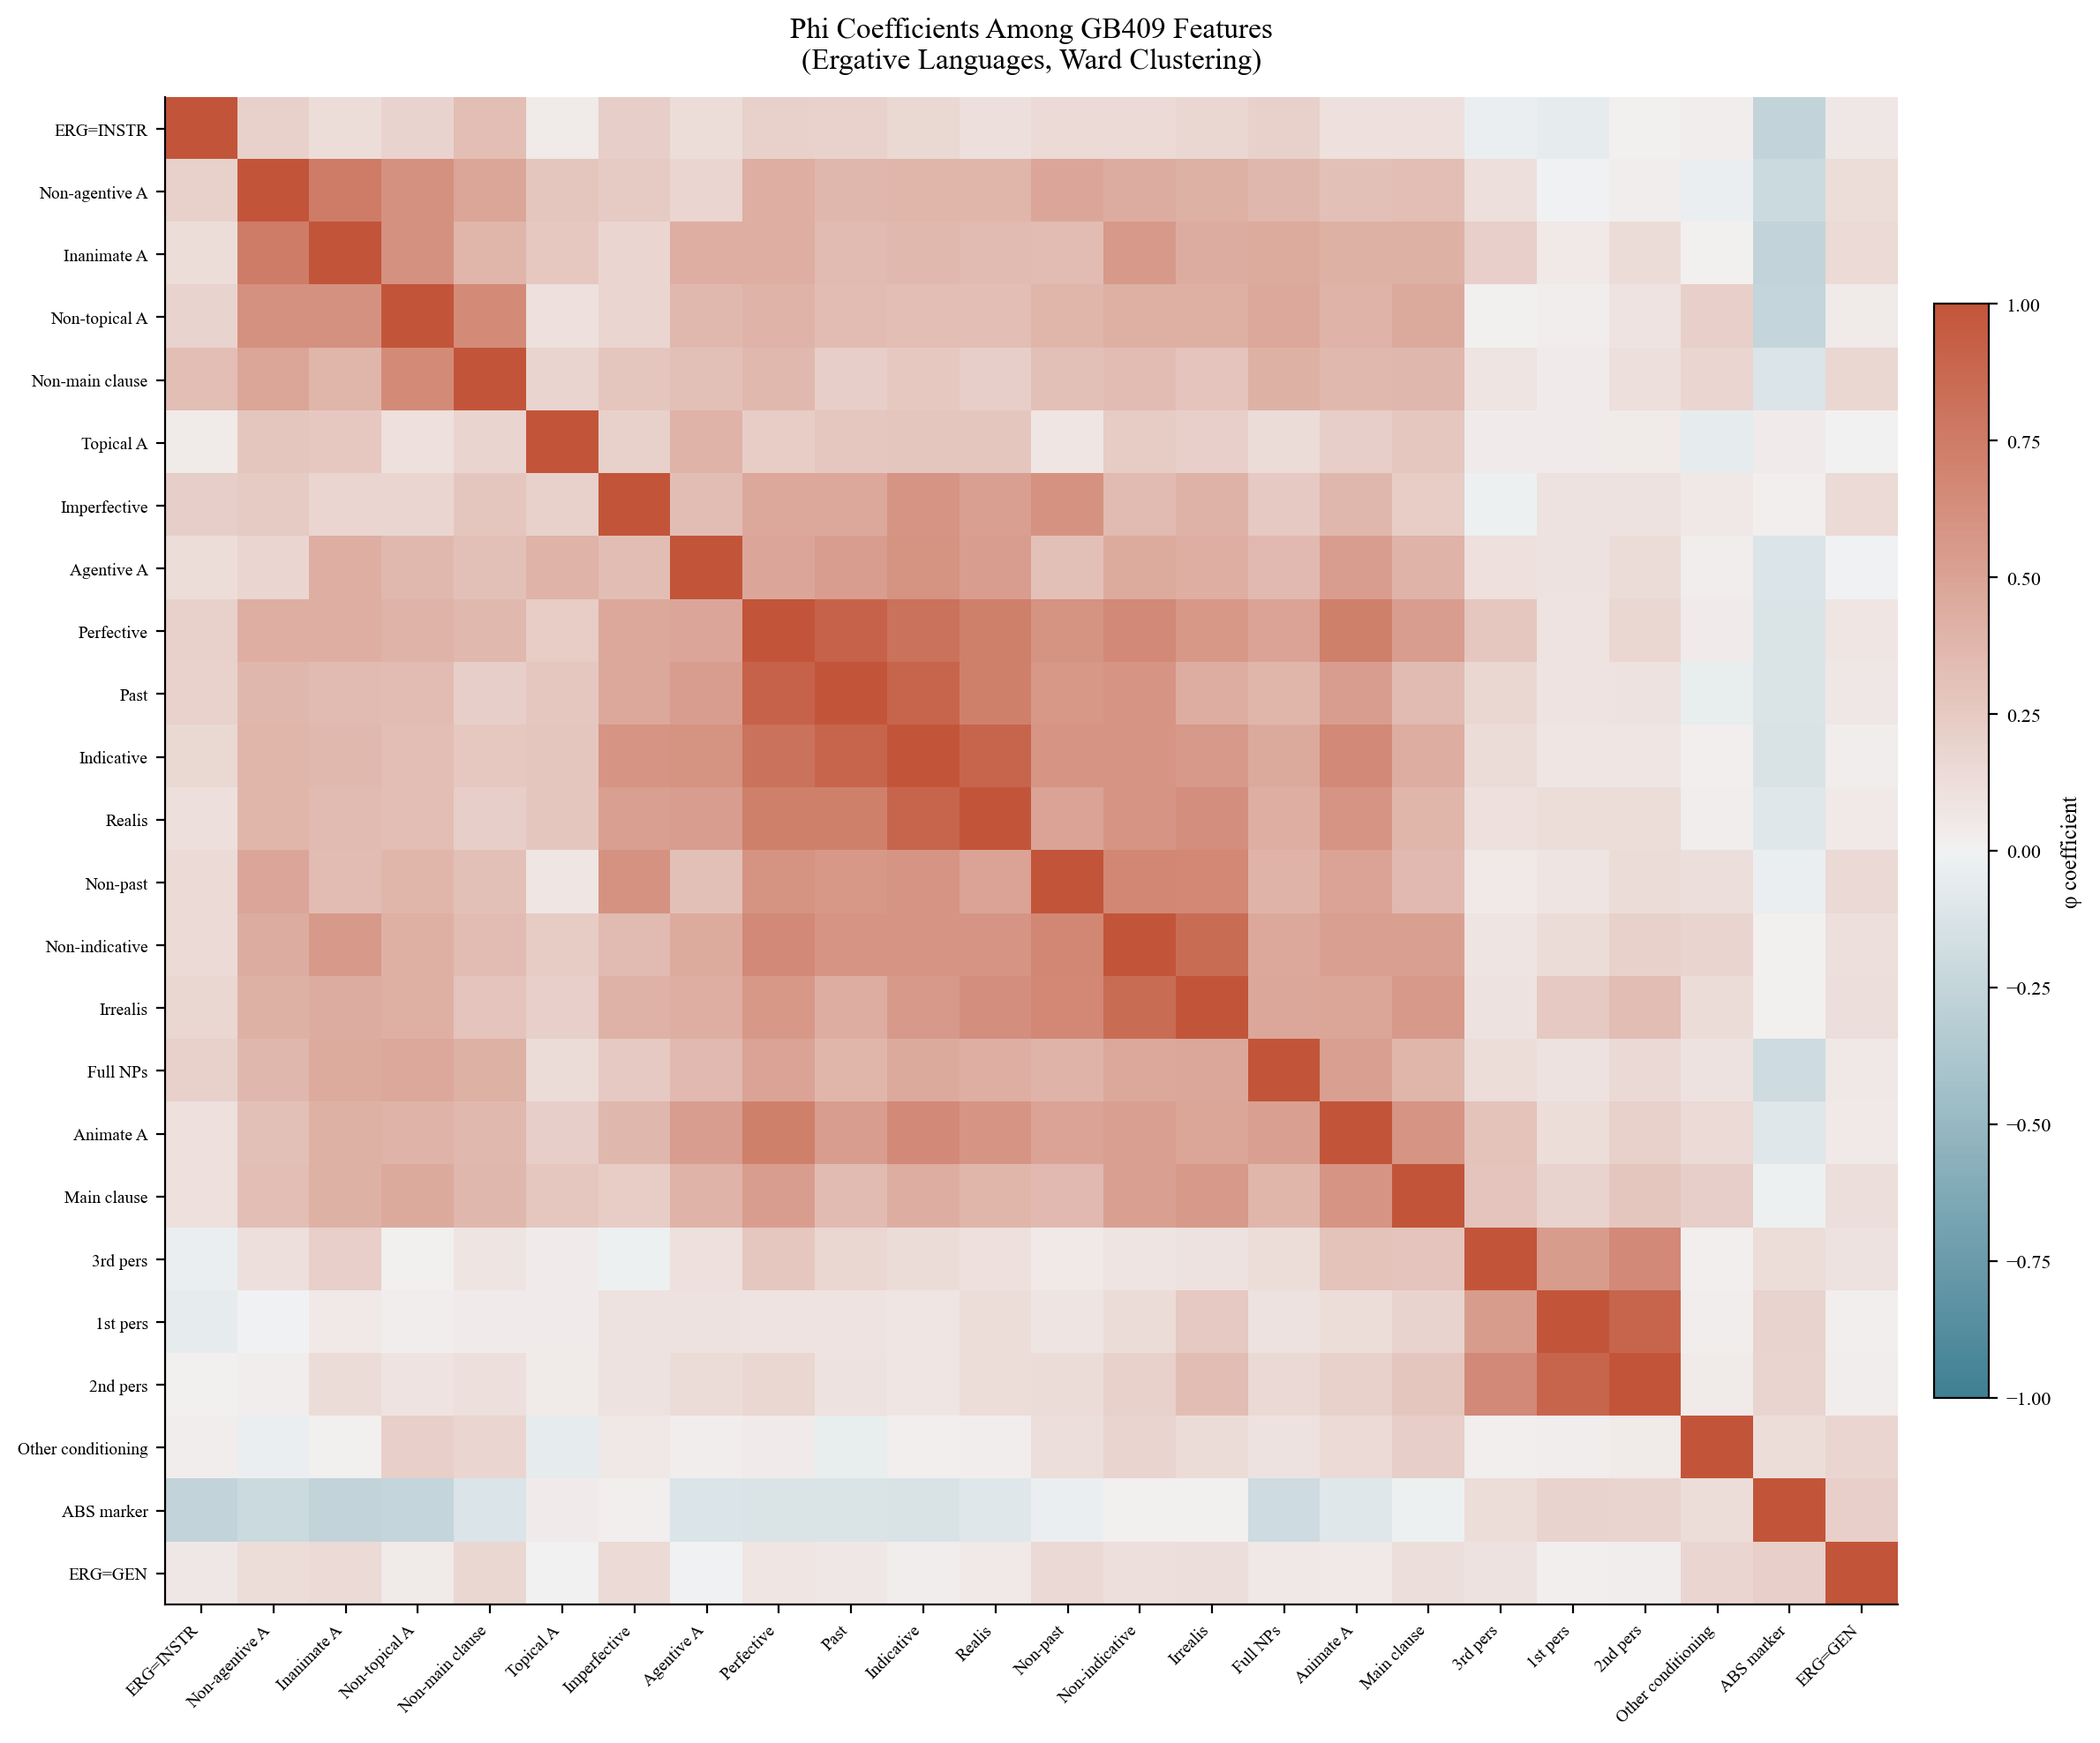
\includegraphics[width=0.88\textwidth]{figA_phi_heatmap.png}
\caption{\textbf{Pairwise feature correlations ($\varphi$ coefficient) across
all 24 ERGON features.} Features are ordered by thematic domain. The
tense/aspect/mood/realis block (GB409\_6--13) shows very high internal
correlations ($\varphi > 0.85$). The person features (GB409\_2--4) form a
second coherent cluster, with lower correlations to GB409\_5 (full NPs),
consistent with the Silverstein hierarchy.}
\label{fig:phi}
\end{figure}

\begin{figure}[H]
\centering

\includegraphics[width=0.92\textwidth]{fig5_silverstein_patterns.png}
\caption{\textbf{Distribution of Silverstein hierarchy patterns.}
Frequency of each implicational pattern category among the 159 ergative
languages with complete data on all four hierarchy features (GB409\_2--5).
The hier4 pattern (ergative marking on all persons and NPs) is by far the
most common (100 languages, 62.9\%), followed by hier3 (NPs only, 23 languages)
and hier2 (3rd person and NPs, 16 languages).}
\label{fig:silverstein_patterns}
\end{figure}

\begin{figure}[H]
\centering

\includegraphics[width=0.92\textwidth]{fig3_families.png}
\caption{\textbf{Distribution of ergative languages across language families.}
Number of ergative languages per family in ERGON ($n = 177$). Trans-Himalayan (43),
Austronesian (33), Pama-Nyungan (24), and Trans-New Guinea (18) are the
most extensively represented families, together accounting for 67\% of the
ergative sample.}
\label{fig:families}
\end{figure}

\end{document}
